\documentclass[12pt]{amsart}

%Below are some necessary packages for your course.
\usepackage{amsfonts,latexsym,amsthm,amssymb,amsmath,amscd,euscript}
\usepackage{graphicx}
\graphicspath{ {./images/} }
\usepackage{framed}
\usepackage{fullpage}
\usepackage{hyperref}
\usepackage{enumitem}
    \hypersetup{colorlinks=true,citecolor=blue,urlcolor =black,linkbordercolor={1 0 0}}

\newenvironment{statement}[1]{\smallskip\noindent\color[rgb]{1.00,0.00,0.50} {\bf #1.}}{}
\allowdisplaybreaks[1]

%Below are the theorem, definition, example, lemma, etc. body types.

\newtheorem{theorem}{Theorem}
\newtheorem*{proposition}{Proposition}
\newtheorem{lemma}[theorem]{Lemma}
\newtheorem{corollary}[theorem]{Corollary}
\newtheorem{conjecture}[theorem]{Conjecture}
\newtheorem{postulate}[theorem]{Postulate}
\theoremstyle{definition}
\newtheorem{defn}[theorem]{{Definition}}
\newtheorem{prob}[theorem]{{Problem}}
\newtheorem{example}[theorem]{Example}

\theoremstyle{remark}
\newtheorem*{remark}{Remark}
\newtheorem*{notation}{Notation}
\newtheorem*{note}{Note}

% You can define new commands to make your life easier.
\newcommand{\BR}{\mathbb R}
\newcommand{\BC}{\mathbb C}
\newcommand{\BF}{\mathbb F}
\newcommand{\BQ}{\mathbb Q}
\newcommand{\BZ}{\mathbb Z}
\newcommand{\BN}{\mathbb N}

% We can even define a new command for \newcommand!
\newcommand{\nc}{\newcommand}

% If you want a new function, use operatorname to define that function (don't use \text)
\nc{\on}{\operatorname}
\nc{\Spec}{\on{Spec}}

\title{CS51, Final Project} % IMPORTANT: Change the problemset number as needed.

\begin{document}

\maketitle

\vspace*{-0.25in}
\centerline{\today}
% Just so that your CA's can come knocking on your door when you don't hand in that problemset on time...

\vspace*{0.15in}

\centerline{\textbf{Report on the extensions of the MiniML interpreter}}
\centerline{}

\begin{enumerate}
	\item \textbf{Changes to the Interpreter}\\
	\\
	For the final project, I decided to modify the parser to allow for syntactic sugar and add extra operations for integer values. I specifically modified the parser to allow let-bound functions to be defined in the form "let f x y = x + y in f 1 3" and for unbound functions to take multiple arguments, for example "fun x y -$>$ x + y." In addition, I added the greater than, greater than or equal, less than or equal, quotient, and mod functions to the syntax of the language.  \\
	
	\item \textbf{Adding syntactic sugar}\\
	\\
	In implementing the syntactic sugar, I modified the parser in miniml parser.mly. In this file, I created two new grammar structures called "sugfun" and "suglet", which would allow functions and let expressions to take in more variables before the arrow (-$>$) or equal (=) signs, respectively. For this to happen, I had to modify the fun inputs so that after the variable, notated as ID, a sugfun expression would come. The sugfun expression can simply be the arrow (-$>$) to what the function evaluates, or another ID followed by another sugfun expression which could now be the arrow (-$>$) to what the function evaluates. This allows the parser to parse a function with any number of variables. Similarly the let and let rec expressions behave in the same way. The parser allows for a suglet expression after the variable (ID). The suglet grammar structure allows for more ID's or an equal sign (=) to indicate to the parser that it should now include what comes after the equal sign in the second part of the data type. In this way, the interpreter parses a function such as "fun x y -$>$ x + y" as "let fun x -$>$ fun y -$>$ x + y" and a let "f x = x + 1 in f 1" as "let f = fun x -$>$ x + 1 in f 1." For the interpreter to work as expected, I had to create a separate grammar structure because after the let or let rec should come a number of variables (ID's) followed by an equal sign and not an arrow (-$>$). If I had implemented it as a single grammar structure, the parser would allow me to interpret expressions like "let f x -$>$ x + 1 in f 3" or "fun x y = x + y," which should instead raise an error.\\
	\\
	\\
	\centerline{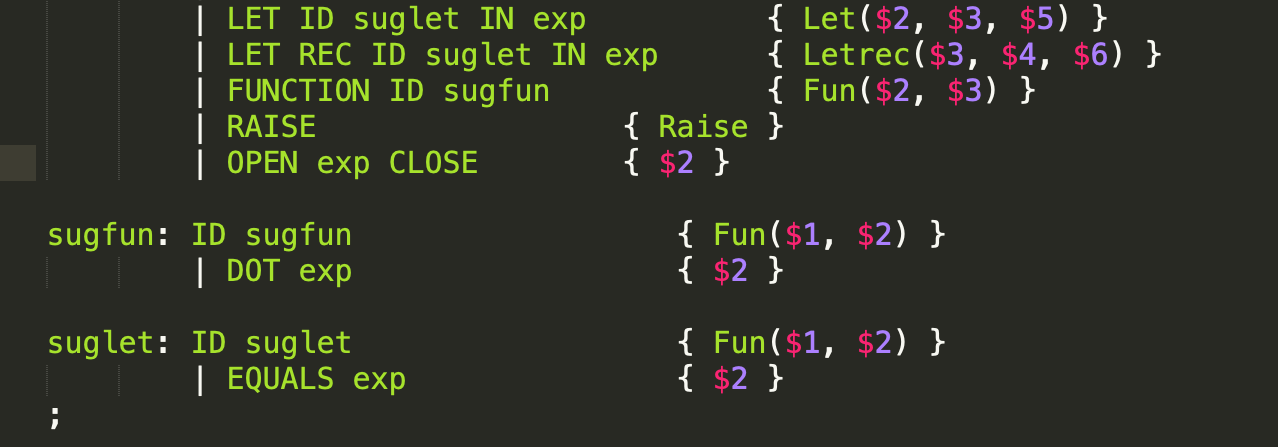
\includegraphics[scale=0.63]{parsercode}}
	\centerline{Figure 1. Code that allows for syntactic sugar in the parsing method.}\\
	\\
	\\
	\centerline{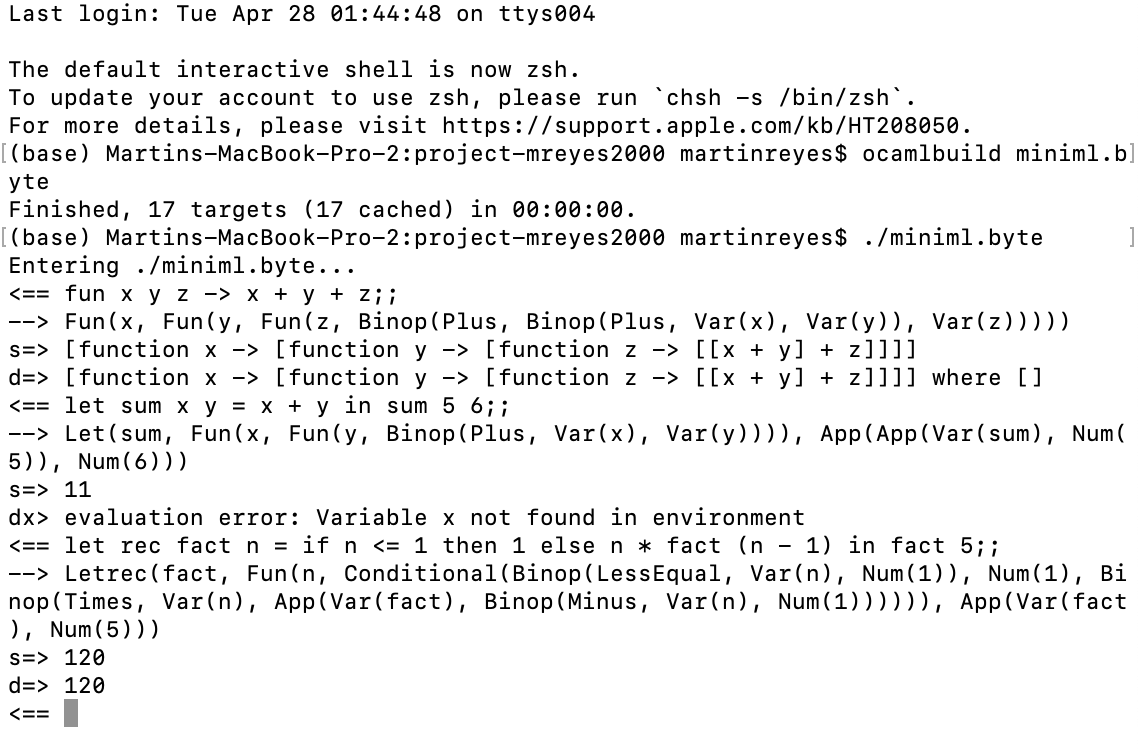
\includegraphics[scale=0.63]{minimlparser}}
	\centerline{Figure 2. The interpreter parsing and evaluating}
	\centerline{three different types of usages of the syntactic sugar.}\\

	\item \textbf{Adding more integer operations}\\
	\\
	In addition to adding syntactic sugar to my interpreter, I also decided to add more binary operations for integers, such as more inequalities and the division and modulus operations. To do this, I had to modify the lexical analyzer in miniml lex.mll, where I defined new symbols such as "$<$=" (less than or equal), "$>$=" (greater than or equal), "$>$" (greater than), "/" (integer division), and "$\%$" (modulus) and assigned them to their tokens. Then, I modified the parser in miniml parser.mlym where I defined the tokens and gave them an algebraic order. Finally, I had to define these operators as new types in expr.mli and implement them in borth expr.ml and evaluation.ml in most of the functions. Luckily, the functions are coded so that one can easily define and implement more types in the functions. \\
	\\
	\\
	\centerline{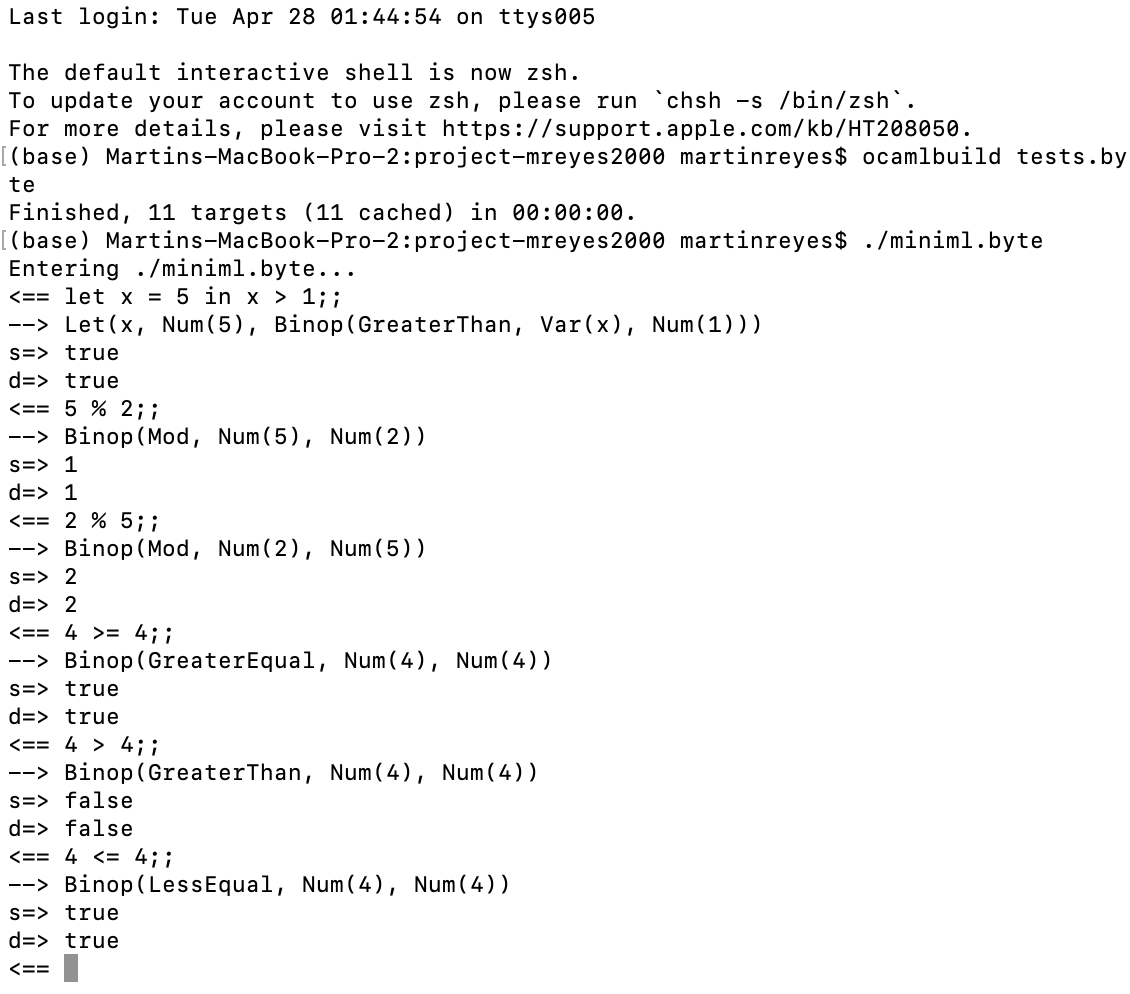
\includegraphics[scale=0.63]{operations}}
	\centerline{Figure 3. The interpreter parsing and evaluating the newly implemented binary operations.}\\
\\
\end{enumerate}

\end{document}
